\documentclass[../main.tex]{subfiles}

\begin{document}

We expect this project to be completed in the fall of 2023. Aim 1 is complete, Aim 2 is largely complete, and Aim 3 has already begun. The full timeline is shown in Figure \ref{timeline}.

\begin{figure}[h!]
  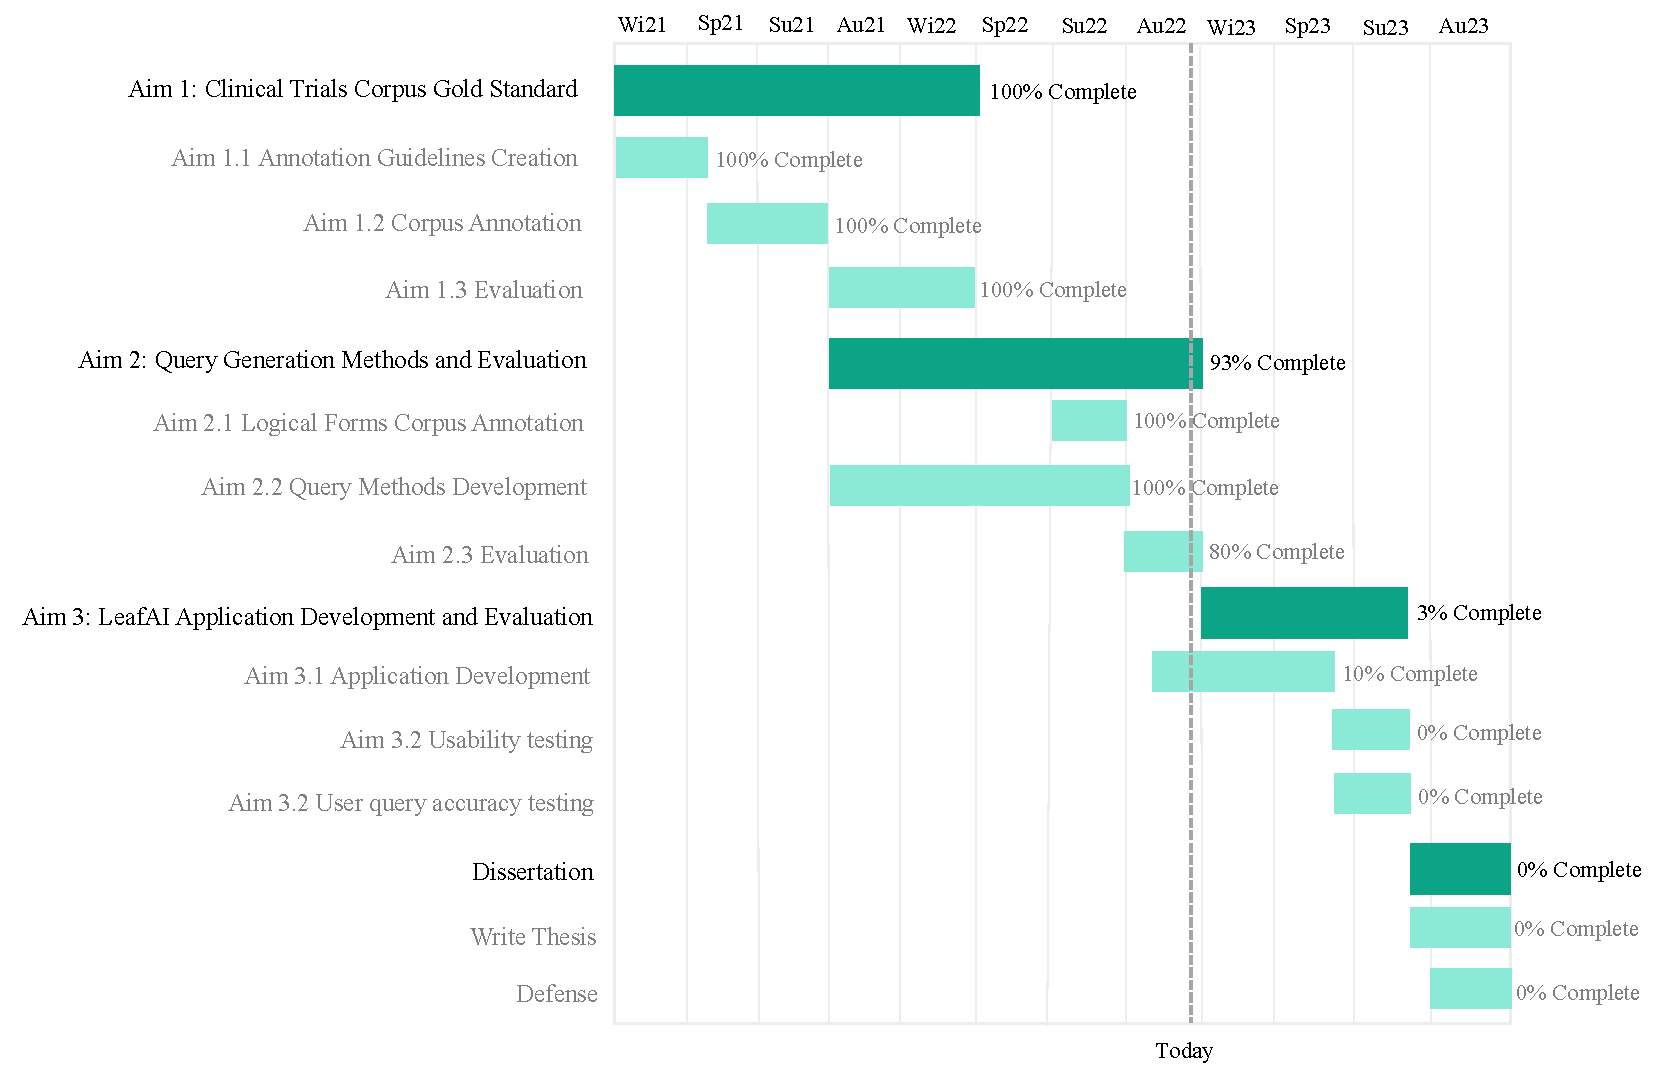
\includegraphics[scale=0.66]{Figures/timeline.pdf} 
\caption{Project completion timeline.}
\label{timeline}
\end{figure}

Clinical trials have a significant impact on biomedical research and the approval of new drugs and methods for treating conditions which affect humans. Finding patients meeting criteria for clinical trials - and biomedical research in general - is often a time-consuming and difficult challenge. This project aims to use NLP and a user-friendly web application to help researchers accomplish this. In Aim 1, we developed the Leaf Clinical Trials corpus, a gold standard for identifying key elements within eligibility criteria. In Aim 2, we developed the Leaf Logical Forms corpus and state-of-the-art methods for generating queries to identify patients meeting eligibility criteria. In Aim 3, we will create an intuitive web application, LeafAI, capable of quickly executing user-defined criteria and transparently explaining its findings.

\end{document}